\section{Introduction}

%------------------------------------------------

\begin{frame}
    \frametitle{Motivation}
    \vspace{3mm}
	  \begin{itemize}
	        \item Breast cancer is one of the leading causes of mortality in women \cite{breast_cancer}.
		\vspace{3mm}
	        \item Identifying molecular subtypes:
			\begin{itemize}
				\item Luminal A
				\item Luminal B
				\item HER2-enriched
				\item Basal-like
			\end{itemize}
			 is key for personalized treatments \cite{b1}.
	           \vspace{3mm}
		 \item Current procedures (biopsies, genomic assays) are invasive, expensive, and time-consuming.
		\vspace{3mm}	        
		\item \textbf{Radiomics}: a non-invasive method that extracts features from MRI images to capture phenotypic traits of the tumor.
	    \end{itemize}
    \vfill 
\end{frame}

%------------------------------------------------

\begin{frame}
    \frametitle{Objectives}
    \vspace{3mm}
	    \begin{itemize}
	        \item \textbf{General Objective:} Develop a non-invasive approach based on MRI images to determine molecular subtypes.
	            \vspace{5mm}
		\item \textbf{Specific Objectives:}
	        \begin{itemize}
	            \item Utilization of the provided radiomic features.
	            \item Incorporation of clinical data.
	            \item Integration of multigenic assay data.
	        \end{itemize}
	    \end{itemize}
\vspace{-4mm}
   \begin{figure}[h]
        \centering
        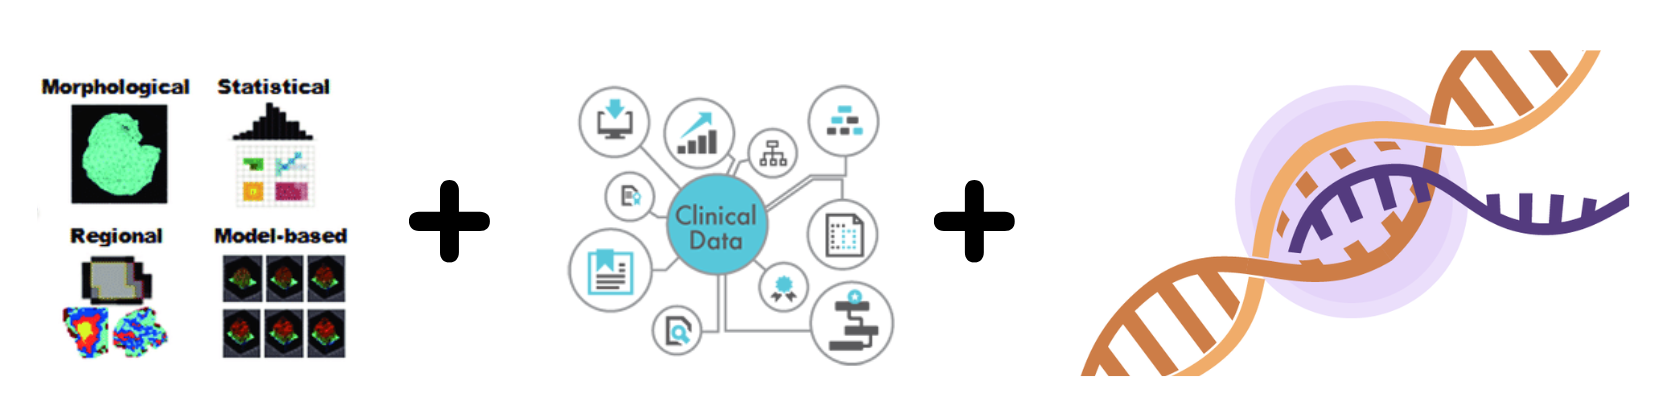
\includegraphics[width=0.9\linewidth]{data.png}
        \label{fig:data_overview}
    \end{figure}

    \vfill 
\end{frame}